\chapter{Edge detection}

In this chapter let us focus on the main goal of the thesis, which is edge detection. An edge is a place where image brightness changes rapidly. There are various methods to identify such discontinuities. The most popular are gradient based (e.g. Canny, Prewitt, Sobel) and Laplacian based. However, there is also another method, which provides similar results and can be more efficient in terms of computation. This method is based on the 2-Dimensional Discrete Wavelet Transform described in section \ref{sec:2D_DWT}. \newline

The mentioned method contains the following steps. \textit{** Link to article Edge detection **}
\begin{enumerate}
\item Convert image to grey scale.
\item Apply 2-D DWT on an image.
\item Remove the LL part.
\item Denoise the LH, HL and HH coefficients.
\item Reconstruct the initial image.
\item Post-processing - modify contrast to emphasize obtained edges.
\end{enumerate}

\section{Implementation of an algorithm}

The algorithm is implemented in \texttt{Python} using \texttt{PyWavelets} package. There are used also auxiliary packages like: \texttt{numpy}, \texttt{matplotlib}, \texttt{PIL} and \texttt{scipy}. The \texttt{PyWavelets} package contains all features required to edge detection algorithm, i.e. 2D Forward and Inverse Discrete Wavelet Transform, build-in many wavelet functions and thresholding functionality (used to denoise coefficients).

Lets go deeper into algorithm, using a simple example - white square on a black background.

\begin{figure}[h]
	\centering
	
\includegraphics[width=0.3\textwidth]{graphs/square.png}
	\caption{An initial image - a white square.}
\end{figure}

Initially, a colour image must be simplified by conversion to grey scale. Edges are recognised as changes in brightness, so a single pixel should contains only information about a colour (black) intensity. Our initial image is already black and white so we do not need to convert it. Now, we can apply the 2D DWT function. As a result, according to the description in section \ref{sec:2D_DWT}, we obtain four components of wavelet coefficients: LL, LH, HL and HH shown on a graph \ref{fig:square_coeffs}. It is clearly visible that the LL part reflects the initial image and the rest components contains information about rapid brightness changes in particular directions. 

\begin{figure}[h]
	\centering
	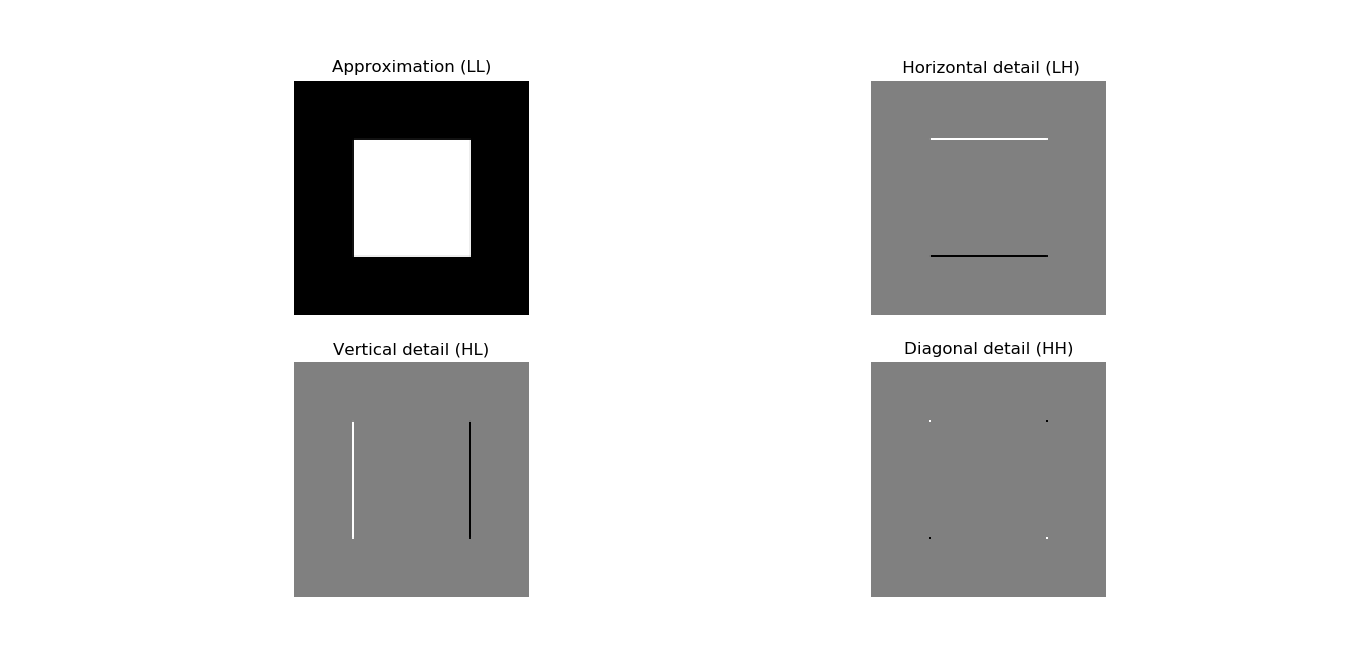
\includegraphics[width=\textwidth]{graphs/square_db2_coeffs.png}
	\caption{2-D DWT coefficients.}
	\label{fig:square_coeffs}
\end{figure}

Thus, we are interested only in components which gives information about edges, so we remove the approximation part - figure \ref{fig:square_coeffs_d}.

\begin{figure}[h]
	\centering
	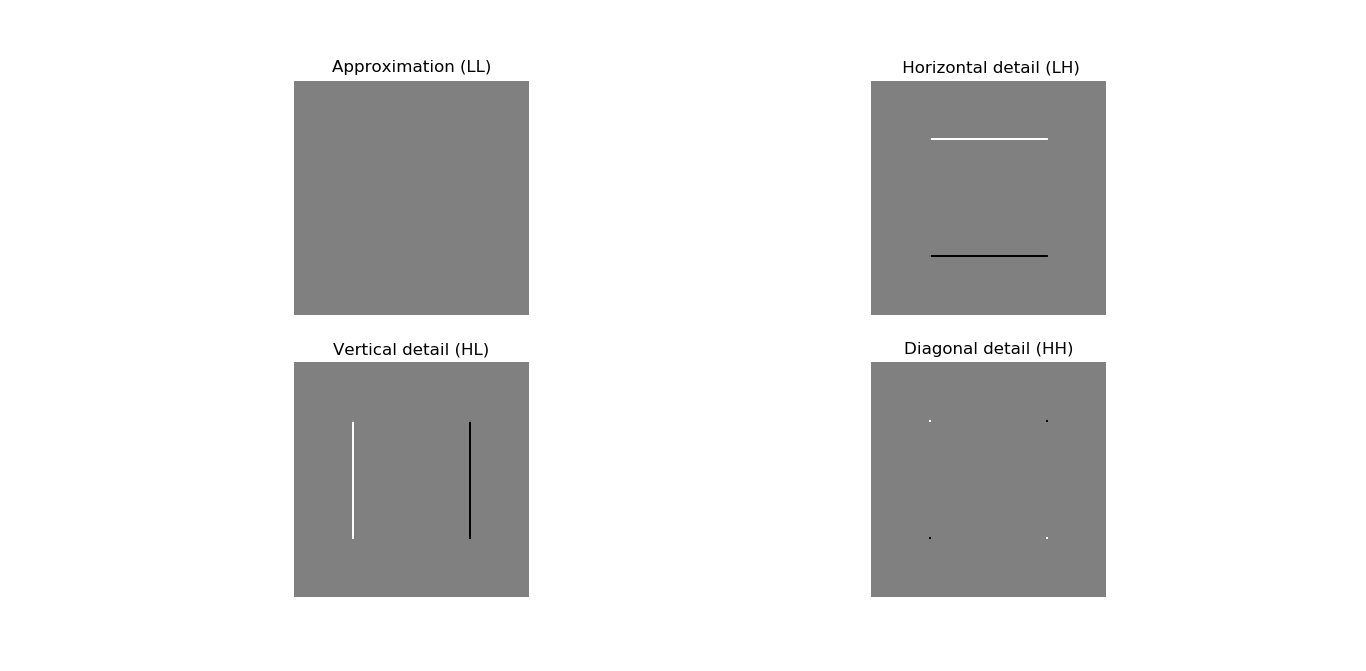
\includegraphics[width=\textwidth]{graphs/square_db2_coeffs_d.png}
	\caption{2-D DWT coefficients with removed the LL part.}
	\label{fig:square_coeffs_d}
\end{figure}

Subsequently, remaining components can be denoised. It means, we can get rid off small, insignificant coefficients by thresholding. More about setting the threshold is described in section \ref{sec:threshold}. This simple example do not require any denoising, so lets go further.

The last main step is reconstruction of the initial image, i.e. application an inverse DWT on the denoised coefficients. In the result, we obtain edges of the initial image presented on a graph \ref{fig:square_idwt}.

\begin{figure}[h]
	\centering
	
\includegraphics[width=0.3\textwidth]{graphs/square_db2.png}
	\caption{A reconstructed image showing the edges.}
	\label{fig:square_idwt}
\end{figure}

At the end, we can manipulate contrast to emphasize obtained lines. Currently, a background has grey colour and the edges are white or black. Therefore, using simple mathematical calculations we can modify image to have black background and white edges. It is enough to get an absolute value, subtract 128 and then scale by multiplying 2 times.

\textit{** Calculations taken from article Edge detection. Maybe add some more about values in an image array **}

Finally, we obtain the edges of the square shown on the figure \ref{fig:square_idwt_pp}.

\begin{figure}[h]
	\centering
	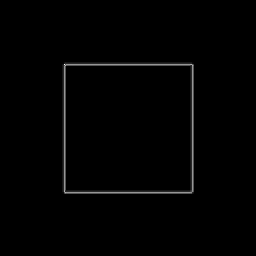
\includegraphics[width=0.3\textwidth]{graphs/square_db2_pp.png}
	\caption{The edges of the square image after post-processing.}
	\label{fig:square_idwt_pp}
\end{figure}

\section{Thresholding}
\label{sec:threshold}
There are two types of thresholding: hard and soft. Lets denote $\lambda$ as threshold value and $d$ as wavelet coefficient. The hard thresholding is defined as follow

\begin{equation}
D^H(d|\lambda)=
\begin{cases}
0, & \text{for } |d| \leq \lambda, \\
d, & \text{for } |d| > \lambda.
\end{cases}
\end{equation}

It assigns zero value for coefficients below the set threshold. The soft thresholding works in the same way on the coefficients smaller than $\lambda$, but additionally the coefficient bigger than the set threshold are ''shrinked'' towards zero, as it is defined below.

\begin{equation}
D^S(d|\lambda)=
\begin{cases}
	0, & \text{for } |d| \leq \lambda, \\
	d-\lambda, & \text{for } d > \lambda, \\
	d+\lambda, & \text{for } d < -\lambda.
\end{cases}
\end{equation}


\subsection{Hard or soft thresholding}

To see the differences between both types of thresholding lets consider a noisy image (fig. \ref{fig:square_s10}).

\begin{figure}[h]
	\centering
	
\includegraphics[width=0.3\textwidth]{graphs/square_s10.png}
	\caption{A noisy square image.}
	\label{fig:square_s10}
\end{figure}

The coefficients of 2-D DWT are shown on the graph \ref{fig:square_s10_coeffs}.

\begin{figure}[h]
	\centering
	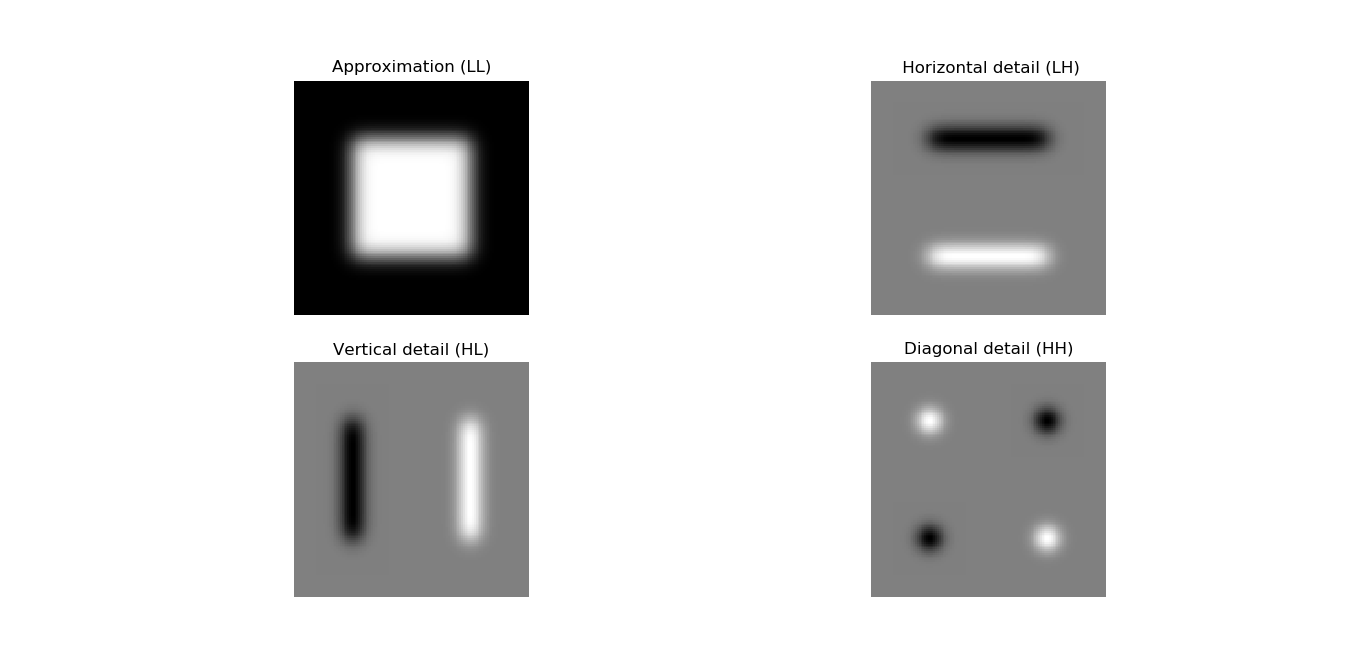
\includegraphics[width=\textwidth]{graphs/square_s10_db1_coeffs.png}
	\caption{2-D DWT coefficients.}
	\label{fig:square_s10_coeffs}
\end{figure}

Now, according to the edge detection algorithm, we remove the LL component and we can denoise the other ones. Results of hard and soft thresholding are presented respectively on a figures \ref{fig:square_s10_hard_coeffs_d} and \ref{fig:square_s10_soft_coeffs_d}.

\begin{figure}[h]
	\centering
	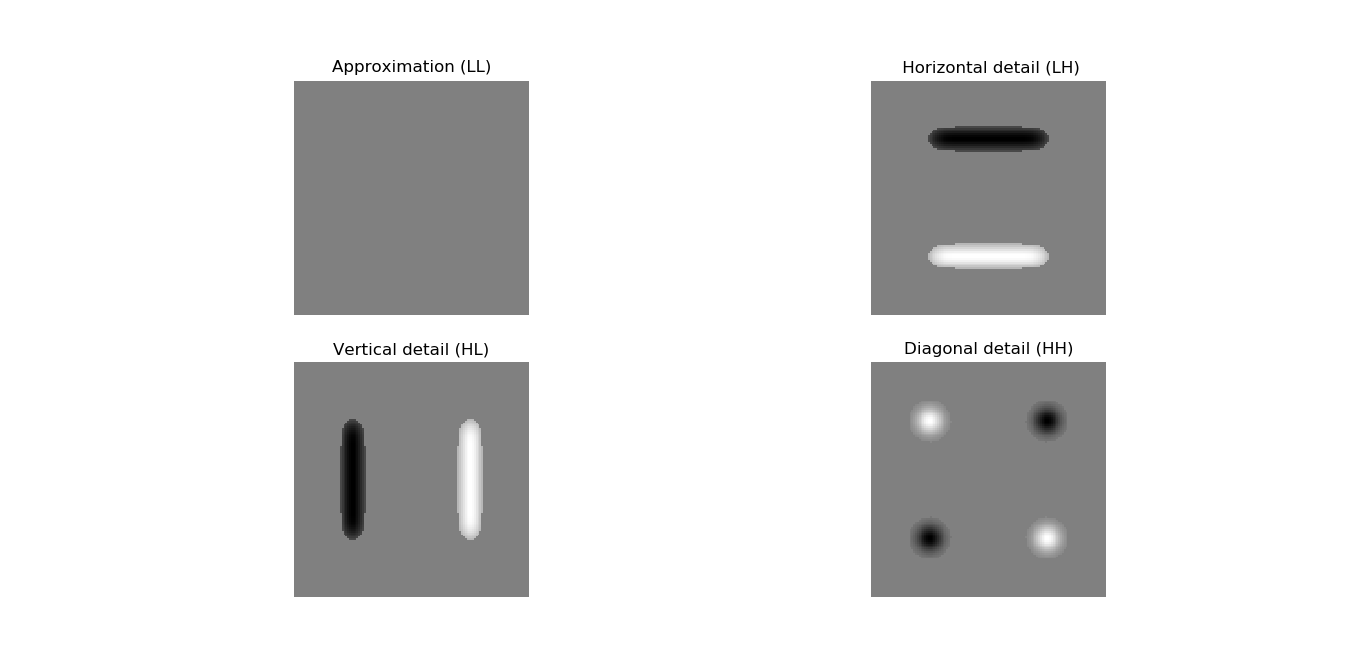
\includegraphics[width=\textwidth]{graphs/square_s10_db1_hard_coeffs_d.png}
	\caption{2-D DWT coefficients after hard thresholding.}
	\label{fig:square_s10_hard_coeffs_d}
\end{figure}

\begin{figure}[h]
	\centering
	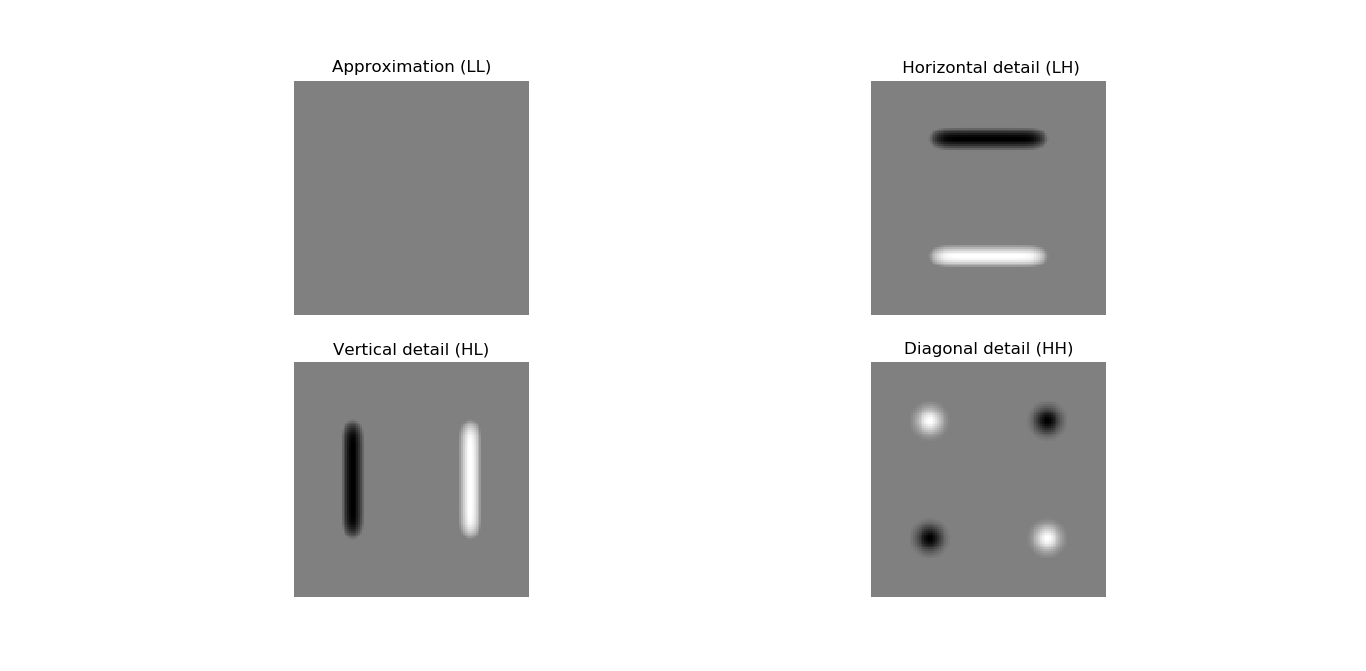
\includegraphics[width=\textwidth]{graphs/square_s10_db1_soft_coeffs_d.png}
	\caption{2-D DWT coefficients after soft thresholding.}
	\label{fig:square_s10_soft_coeffs_d}
\end{figure}

We can see the distinction between both thresholding, especially on the LH and HL components. After soft one the lines are smoother and slightly narrower, then in the other case. Therefore, the soft thresholding seems to be better for edge detection. Because of the smoother results, it is especially useful for the real life images, where edges are often blurred. To confirm this conclusion lets compare the final results, after inverse DWT (fig. \ref{fig:square_s10_idwt_pp})

\begin{figure}[h]
	\begin{subdiagrams2}{square_s10_db1_hard_pp}{hard}{square_s10_db1_soft_pp}{soft}
	\end{subdiagrams2}
	\centering
	\caption{Results of edge detection with hard and soft thresholding.}
	\label{fig:square_s10_idwt_pp}
\end{figure}

\subsection{Setting the threshold}
The corollary from the previous subsection is that the soft thresholding provides better results for edge detection. However, there is also a question how to choose the value of a threshold $\lambda$ to denoise coefficients and do not loose any significant information. A simple idea is to get a quantile of the coefficients in the specific components. 

\textit{** Add histograms of the coefficients **}

We decided to start with a quantile on level 0.95. It occurs to be accurate for the majority of standard images. All the earlier results are computed for threshold set as 0.95 quantile. Although, images which are noisier could require changing the quantile level.

Lets consider three images of basic diamond shape with different noisiness, shown on the figure \ref{fig:diamonds}.

\begin{figure}[h]
	\begin{subdiagrams3}{diamond_s16}{}{diamond_s10}{}{diamond_s4}{}
	\end{subdiagrams3}
	\centering
	\caption{The initial images of diamond with different noise level.}
	\label{fig:diamonds}
\end{figure}

At first, see how looks the result with mentioned earlier threshold set as 0.95 quantile (fig. \ref{fig:diamonds_95}). Algorithm found the edges properly but they are quite wide, especially for the noisier image. Lets try to increase the threshold to quantile on the 0.99 level. The results are presented on the graph \ref{fig:diamonds_99}. It can be seen that for (b) and (c) images the edges are narrower and visible. Nevertheless, result for the (a) image is incorrect, threshold is too high and too much information is removed. Hence, lets consider one more threshold on a 0.98 quantile level. The recognised edges for (a) and (b) images are presented on the figure \ref{fig:diamonds_98}. For this threshold edges are correctly detected.

In conclusion, for noisier images the increased threshold provides more accurate result, but increasing the threshold must be done carefully to not ignore crucial informations. Additionally, when image have one sharp object and noisy background, increasing the threshold we can control the amount of background details in the result.

\begin{figure}[h]
	\begin{subdiagrams3}{diamond_s16_db1_95_pp}{}{diamond_s10_db1_95_pp}{}{diamond_s4_db1_95_pp}{}
	\end{subdiagrams3}
	\centering
	\caption{The recognized edges for the diamonds with $\lambda$ equals 0.95 quantile.}
	\label{fig:diamonds_95}
\end{figure}

\begin{figure}[h]
	\begin{subdiagrams3}{diamond_s16_db1_99_pp}{}{diamond_s10_db1_99_pp}{}{diamond_s4_db1_99_pp}{}
	\end{subdiagrams3}
	\centering
	\caption{The recognized edges for the diamonds with $\lambda$ equals 0.99 quantile.}
	\label{fig:diamonds_99}
\end{figure}

\begin{figure}[h]
	\begin{subdiagrams3}{diamond_s16_db1_98_pp}{}{diamond_s10_db1_98_pp}{}{diamond_s4_db1_98_pp}{}
	\end{subdiagrams3}
	\centering
	\caption{The recognized edges for the diamonds with $\lambda$ equals 0.98 quantile.}
	\label{fig:diamonds_98}
\end{figure}


\section{Selection of a wavelet type}

\textit{** Show results for different wavelet types: haar and db2? **}